\chapter{Informationsbeschaffung}
\label{Informationsbeschaffung}
 In einer ersten Phase wurde ein Zeitraum zur Informationsbeschaffung festgelegt. Dieser Abschnitt ist einerseits für die Themeneinarbeitung und anderseits für die Abgrenzung der Aufgabe und der Ziele erforderlich.

Nachfolgend werden die wichtigsten Erkenntnisse der Informationsbeschaffung erläutert, die maßgebend für die Konzeption in Kapitel \ref{chap:Konzeption} und die Realisierung in Kapitel \ref{chap:Realisierung} sind. Dabei werden zu einzelnen Komponenten und Verfahren Stellung genommen und eruiert, ob diese sich für das Projekt eignen. Des Weiteren werden relevante Software erläutert, welche für die Realisierung nötig sind. Ein weiterer Abschnitt behandelt bereits bestehende Lösungen, die den Stand der Technik aufzeigen.

\section{Entfernungsmessung}
\label{sec:Entfernungsmessung}
In diesem Unterkapitel wird der bestehende 3D-Laserscanner Velodyne VLP-16 analysiert. Dabei werden wichtige Spezifikationen erläutert. Anhand der Spezifikationen und Schnittstellen des Velodyne werden in den nächsten Unterkapitel weitere Komponenten eruiert.   

\subsection{Velodyne VLP-16 Puck}
\label{subsec:Velodyne}
Beim Velodyne VLP-16 Puck handelt es sich um einen Echtzeit 3D-Laserscanner, der auf dem \ac{LIDAR}-Verfahren basiert. Nachfolgende Angaben entstammen dem Datenblatt, wenn nicht anders referenziert. \protect\cite{velodyne}

Der VLP-16 bietet insgesamt 16 Laser-/Detektorpaare, die in Abbildung \ref{fig:angleVLP} ersichtlich sind. Mit diesen wird in horizontaler Lage eine Messbereich von 360$^\circ$  erreicht. Dies wird dadurch ermöglicht, dass der Laserscanner sich intern mit 5 - 20 Rotationen pro Sekunde um die eigene Achse dreht. Die Rotationsgeschwindigkeit ist einstellbar. Dabei wird mit einer horizontalen Auflösung von 0.1$^\circ$ – 0.4$^\circ$ gerechnet. Diese Auflösung begründet sich auf die nötige Zeit eines Messdurchgangs. Um alle 16 Laser abzufeuern und wieder zu entladen dauert es 56 $\mu$s.
Da die 16 Laser mit je 2 $^\circ$ Unterschied ausgerichtet sind ergibt sich daraus eine vertikalen Messbereich von 30$^\circ$ mit einer vertikalen Auflösung von 2$^\circ$. Ein wichtiger Punkt ist somit, dass im stationären Zustand zwischen den Laserstrahlen keine Messpunkte ermittelt werden können. Um dies zu ermöglichen, muss der Laserscanner seine Position verändern können.

\begin{figure}[H]
	\centering
	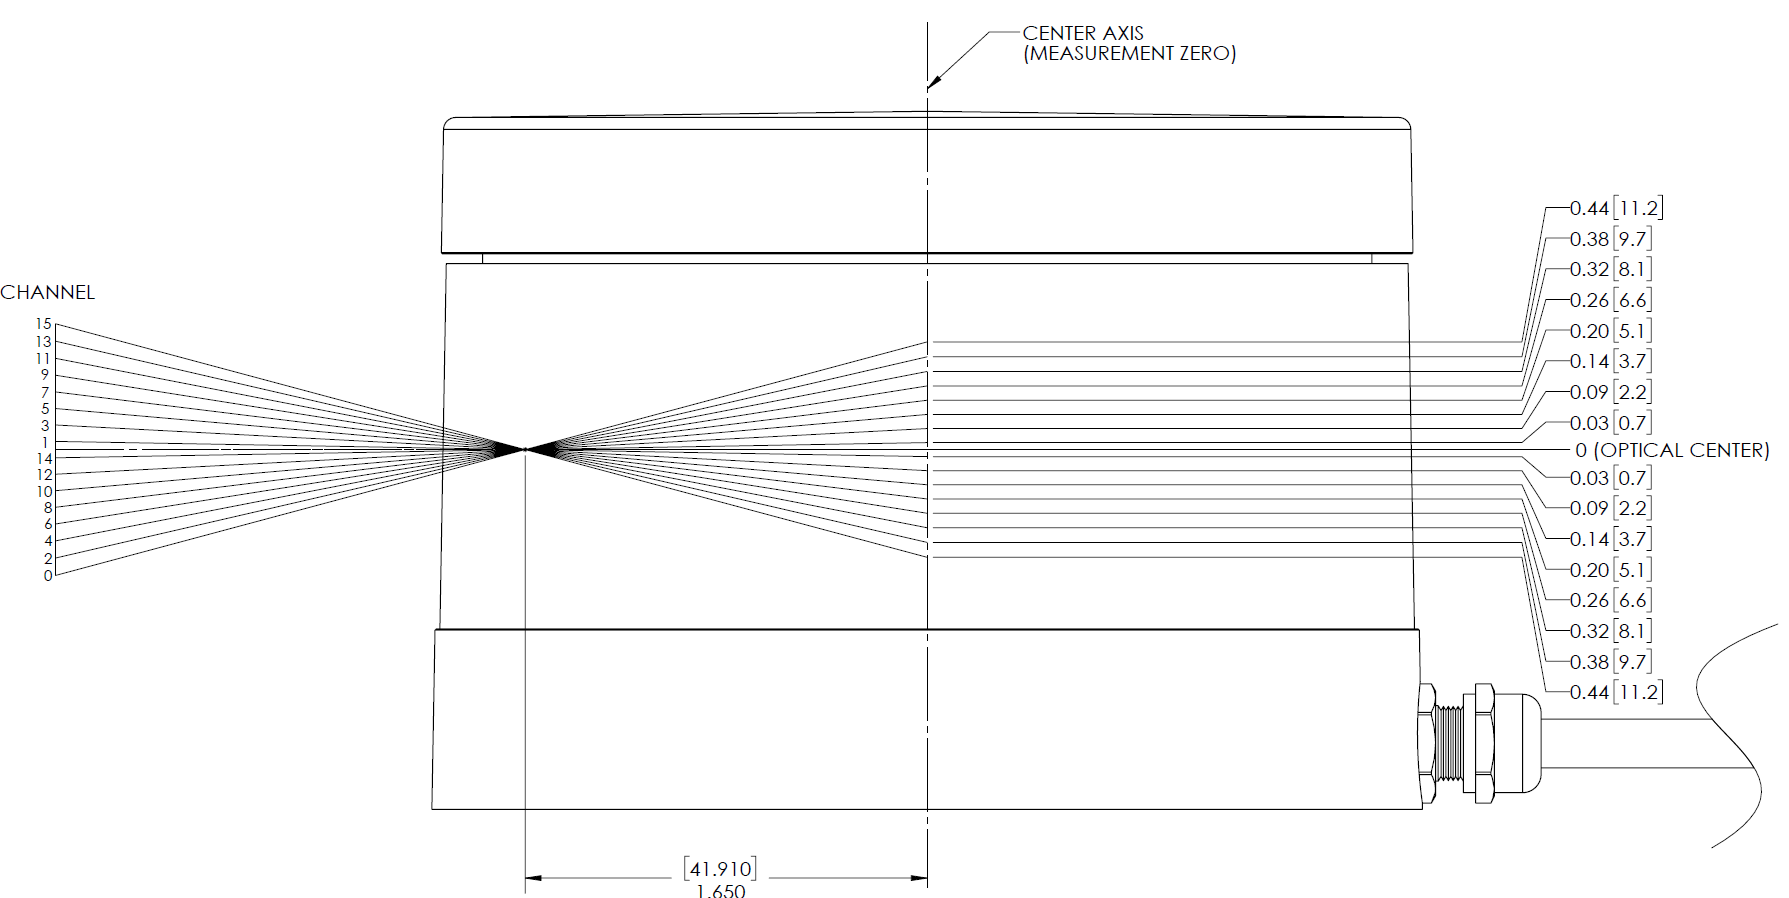
\includegraphics[width=0.6\textwidth]
	{resources/velodyne_channels.PNG}
	\caption[Laserstrahlen des Velodyne  VLP-16]{Laserstrahlen des Velodyne  VLP-16} \protect\cite{velodyne}
	\label{fig:angleVLP}
\end{figure}

Ein relevante Eigenschaft dieses Laserscanners ist die grosse Messdistanz, die Distanzen zwischen 0.43 m bis 100 m ermöglicht. Dabei ist die die typische Toleranz +/- 3 cm. Der Reflektionsgrad wird in 256-bit Auflösung angegeben, d.h. dass der Sensor aus der zurückgesendeten Laserimpulsen die Intensität messen kann.

Der VLP-16 benötigt eine separate Interface Box, mit der die Speisung und die Datenschnittstellen zu einem 8-adrigen Kabel zusammengeführt werden. In Abbildung \ref{fig:CablePin} ist dieses Kabel mit Pinbelegung dargestellt. Dabei werden die Adern 1-4 für die Ethernet Datenübertragung benötigt. Die Adern 5 und 6 sind nur bei zugeschaltetem \ac{GPS} nötig, ansonsten sind diese unbenutzt. Die stabilisierte 12 Volt Spannung wird über die Adern 7 und 8 zugeführt.

\begin{figure}[H]
	\centering
	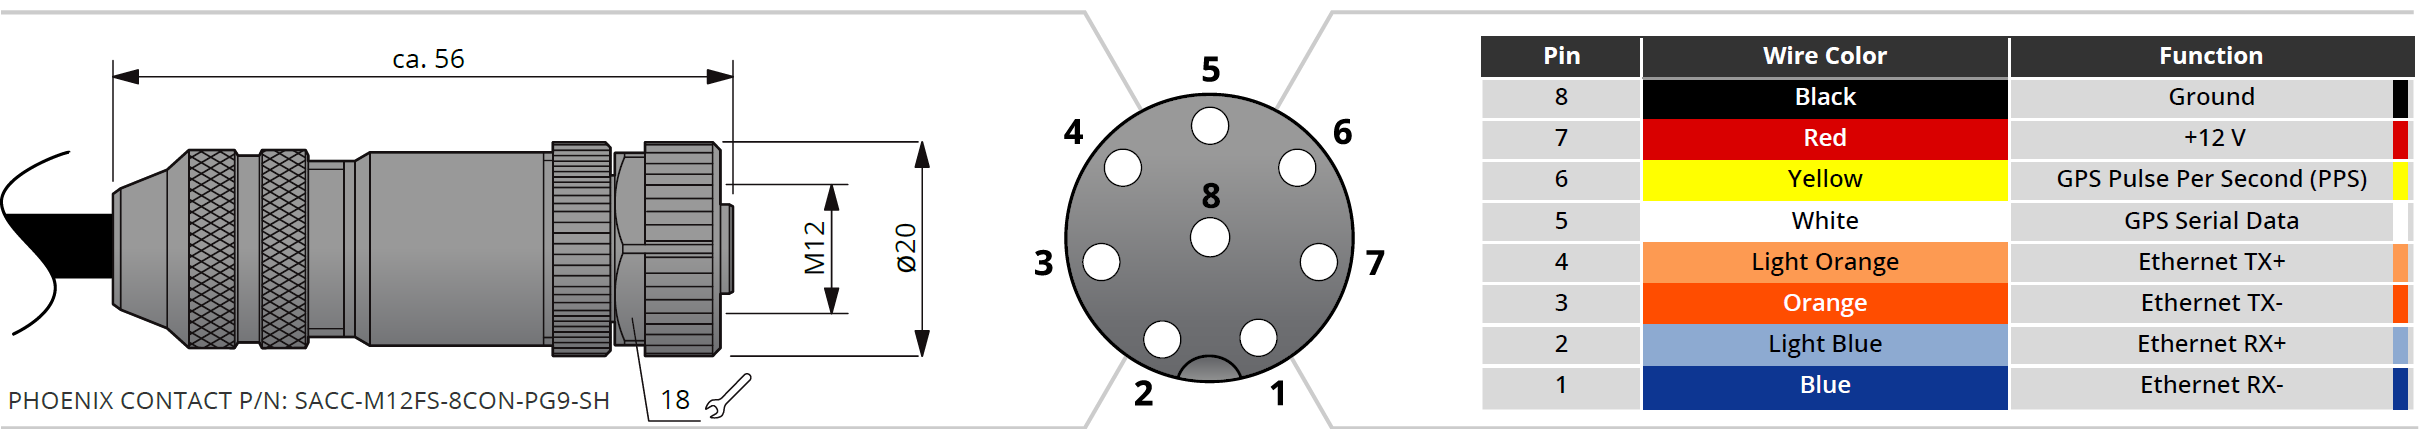
\includegraphics[width=1\textwidth]{resources/Cablepins.PNG}
	\caption[Anschluss und Kabelbelegung]{Anschluss und Kabelbelegung}\protect\cite{velodyne}
	\label{fig:CablePin}
\end{figure} 

Die Interface Box ist in Abbildung \ref{fig:InterfaceBox} ersichtlich. Diese besitzt folgende Anschlüsse; eine 12 Volt Speisung,eine Ethernet RJ45-Anschluss und eine \ac{GPS} Schnittstelle. Für die typische Leistungsaufnahme des Sensors wird 8 Watt angegeben. 

\begin{figure}[H]
	\centering
	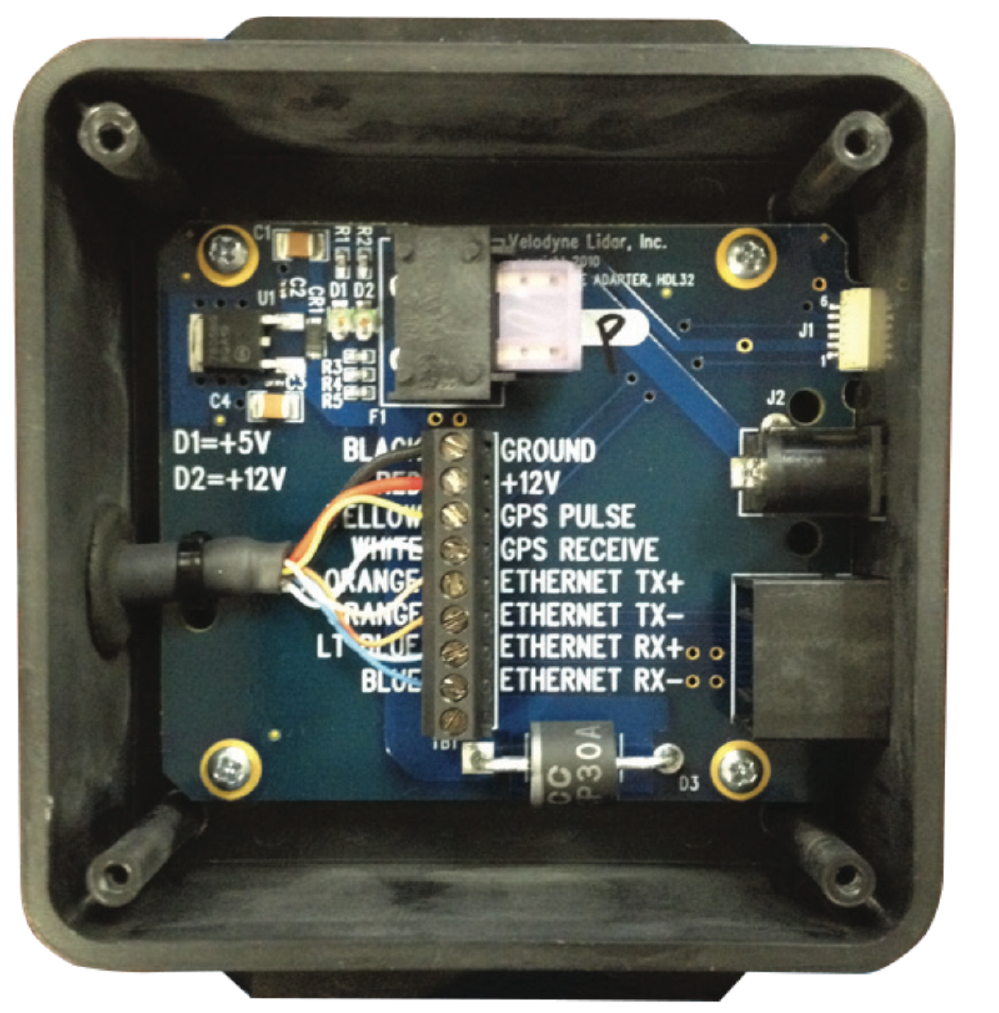
\includegraphics[width=0.4\textwidth]
	{resources/InterfaceBox.PNG}
	\caption[Ansicht auf die Interfacebox]{Ansicht auf die Interface Box} \protect\cite{velodyne}
	\label{fig:InterfaceBox}
\end{figure}

Über die 100 Mbps Ethernetverbindung werden die Daten- und Positionspakete vom Velodyne an den Computer übermittelt. Dabei werden für die zwei verschiedenen \ac{UDP} Pakets die Ports 2368 und 8308 gebraucht. Nachfolgend wird in Abbildung \ref{fig:datapakets} der Aufbau eines Datenpakets dargestellt. Jedes Paket besitzt einen 42-Byte Header und einen Datenblock, der aus Laserrückgabewert, kalibrierten Reflektionsgrad, Azimutwert und Zeitstempel besteht.

\begin{figure}[H]
	\centering
	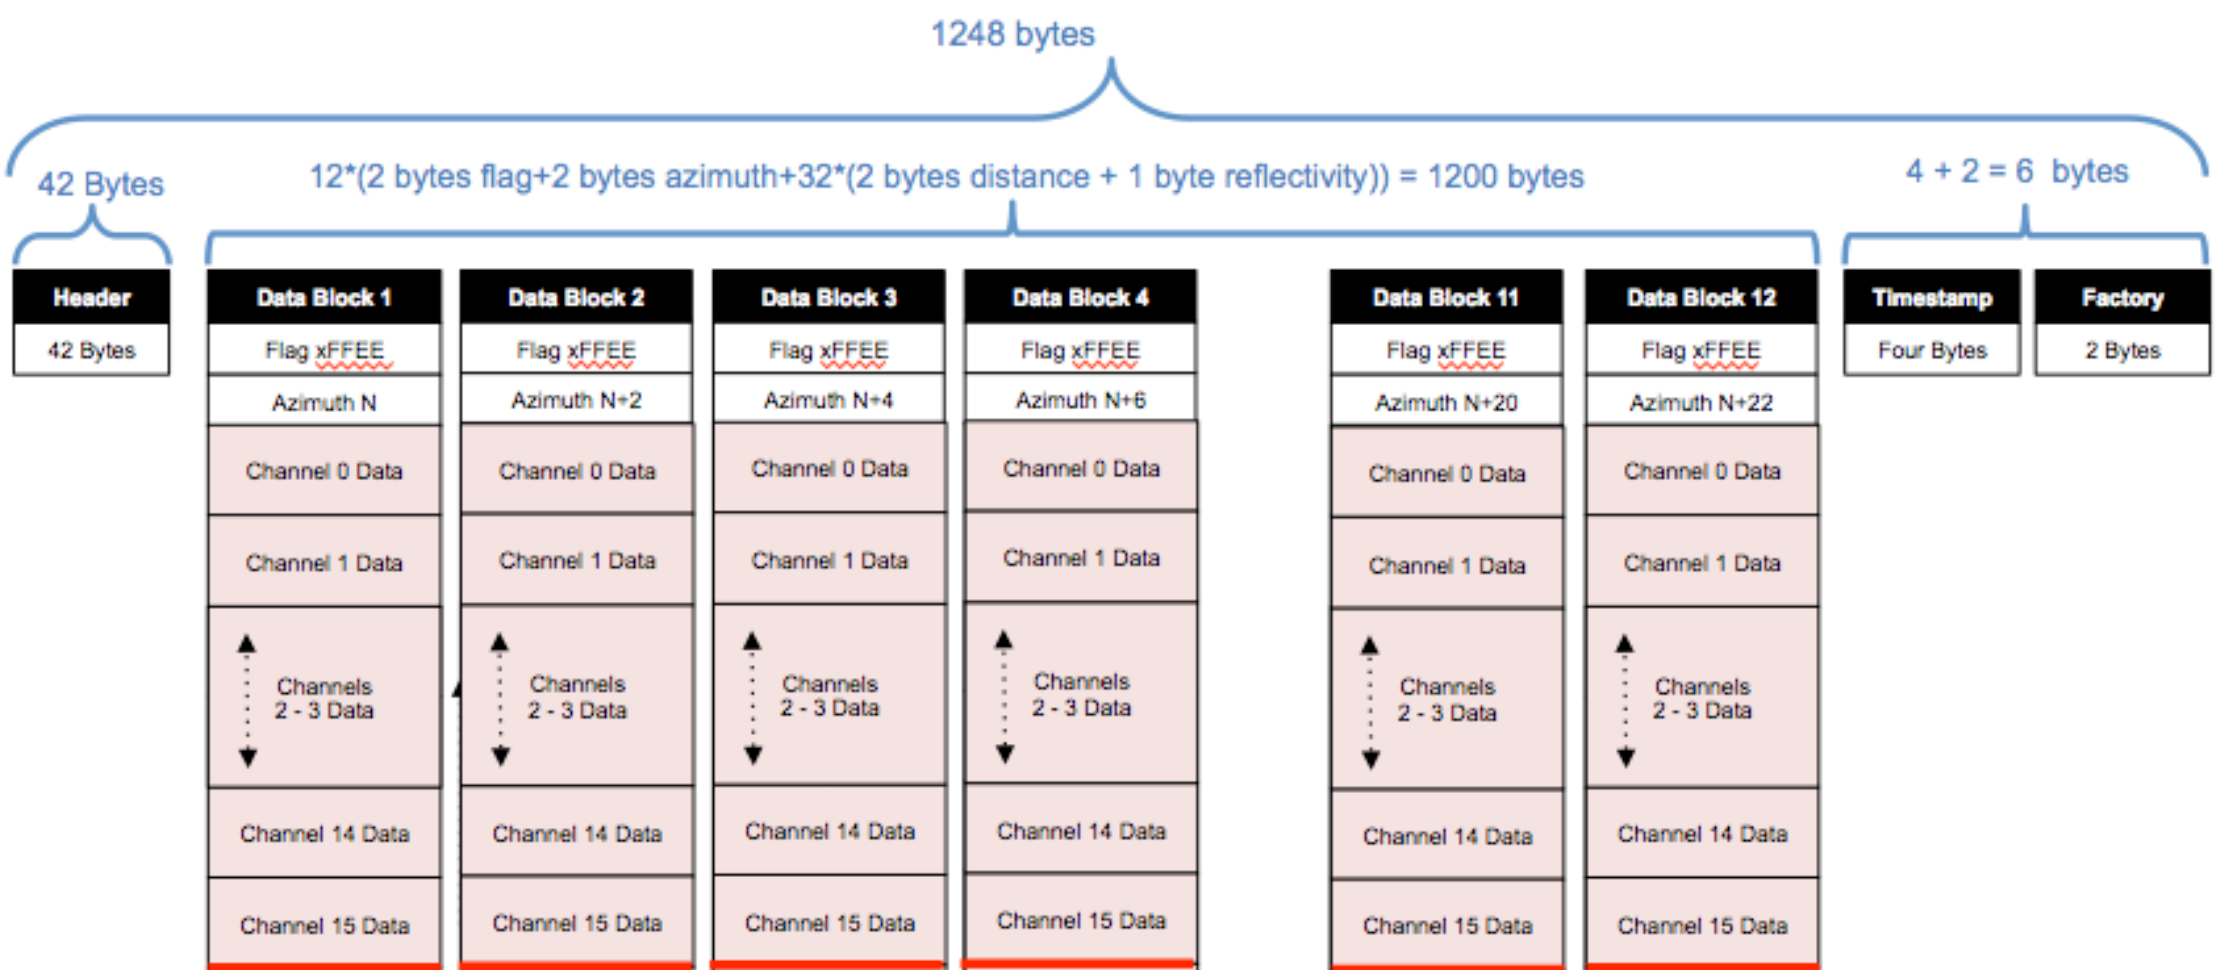
\includegraphics[width=1.0\textwidth]
	{resources/datapakets.PNG}
	\caption[Aufbau Datenpaket]{Aufbau Datenpaket} \protect\cite{velodyne}
	\label{fig:datapakets}
\end{figure}


\section{Stand der Technik}
 \label{sec:Vorzeigeprojekte}
 Dieses Kapitel dient als Vorstudie über den Einsatz des Velodyne VLP-16 durch bereits bestehende Projekte. Dabei werden zwei verschiedene Konfigurationen betrachtet und dazu entsprechend Vor- und Nachteile erläutert. Es handelt sich hierbei um zwei Teams, welche an der \ac{EnRicH} 2017 teilgenommen haben und als State-of-the-Art betrachtet werden.
 
 \subsection{IMM MSAS Team MSS Warschau}
 	\label{subsec:IMM}
Das Institute of Mathematical Machines (IMM) in Warschau hat den Velodyne VLP-16 an einer endlos drehenden Konstruktion befestigt. Dabei ist der Sensor nicht in der üblichen Lage (Ausrichtung XY-Ebene), sondern um 90$^\circ$ abgedreht (Ausrichtung YZ Ebene). In Abbildung \ref{fig:imm} ist die entsprechende Konfiguration abgebildet. 

   \begin{figure}[H]
	\centering
	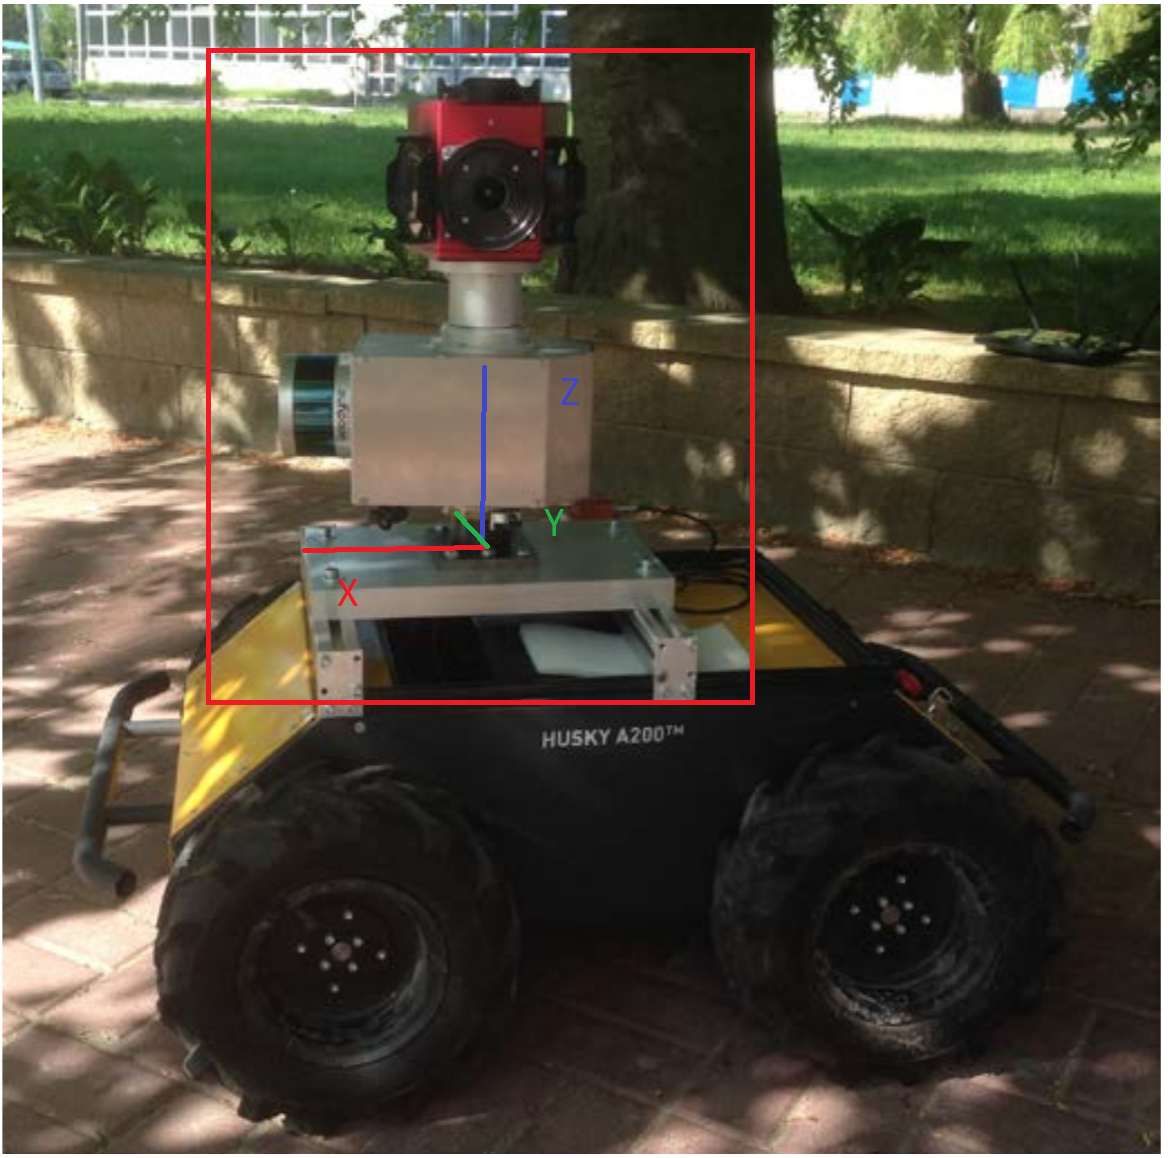
\includegraphics[width=0.6\textwidth]
	{resources/IMM_cop.PNG}
	\caption[Roboter des Team IMM EnRicH]{Roboter des Team IMM an der EnRicH} \protect\cite{IMM}
	\label{fig:imm}
\end{figure}

In der nachfolgenden Betrachtung wird vom Koordinatensystem in der Abbildung \ref{fig:imm} ausgegangen.
Das Team nutzt bei dieser Konfiguration die begrenzte Auflösung des Sensors besser aus. Die vertikale und horizontale Auflösung wechseln dabei. Ist die Konstruktion nicht drehend, kann er in der Vertikalen den Bereich 360$^\circ$ mit der Auflösung von 0.01$^\circ$ - 0.04$^\circ$ messen. In der Horizontalen kann der Bereich 30$^\circ$ mit 2$^\circ$ aufgelöst werden. 

Der Vorteil dieser Konfiguration wird jedoch erst durch die Rotation um die Z-Achse deutlich. Wird der Sensor nun kontinuierlich um die Z-Achse gedreht, verschieben sich die 16 horizontalen Laserstrahlen mit der Umdrehungsgeschwindigkeit der Konstruktion. Einerseits bewegt sich der 30$^\circ$ grosse Messkegel durch den Raum und kann somit 360$^\circ$ in der Horizontalen vermessen. Anderseits kann durch die interne Rotation des Sensors 360$^\circ$  in der Vertikalen ausgemessen werden. Die schlechtere Auflösung von 2$^\circ$ kann somit kompensiert werden. Dies Konfiguration ermöglicht eine detaillierte Messung, da jeder Punkt im Raum von 16 Laserstrahlen mit der Auflösung zwischen 0.1$^\circ$ 0.4$^\circ$ durchlaufen wird. 

Die oben erläuterte Betrachtung gilt jedoch nur, wenn die Umdrehungsgeschwindigkeit der Konstruktion bedeutend langsamer als die interne Umdrehungsgeschwindigkeit des Sensor ist. Ansonsten besteht die Gefahr, dass die Reflektion des Laserstrahls nicht detektiert werden kann. Die Auflösung ist direkt von der Umdrehungsgeschwindigkeit abhängig. Es wird zusätzlich davon ausgegangen, dass keine Translation, d.h. Bewegung des Roboters, stattfindet. Diese Konfiguration eignet sich somit, wenn das zu vermessende Gelände bekannt ist. Dadurch können vordefinierte Positionen angesteuert werden, an denen eine halbe Umdrehung ausreicht, um eine räumliche Messung an der definierten Position zu erstellen. 

Weiter wird in obigen Betrachtung die Abweichung zur Drehachse komplett vernachlässigt. Es entsteht ein Messfehler, der dem Abstand  des Sensors zur Drehachse entspricht. Ein weiterer Messfehler kann durch Translation entstehen, wenn sich das Fahrzeug bewegt. Diese zwei Messfehler lassen sich jedoch durch geometrische Transformation in ein festes Koordinatensystem kompensiert. Die Schwierigkeit dabei ist, die exakten Messewerte mittels einem Drehencoder und einer \ac{IMU} zum jeweiligen Zeitpunkt zu ermitteln. In der nachfolgenden Matrix werden die Variablen der Translation mit t, Skalierung mit s und die Drehung um die Z-Achse mit dem Winkel $\alpha$  angegeben. 
\begin{center}

$\begin{bmatrix}
\centering
\label{fig:TFmatrix}
&s_x * cos\alpha  &s_x*-sin\alpha   &0 &t_x \\ 
&s_y*sin\alpha   &s_y*cos\alpha  &0 &t_y \\ 
&0  &0 &s_z &t_z \\ 
&0  &0  &0 &1 
\end{bmatrix} *\begin{bmatrix}
&x'  \\ 
&y'  \\ 
&z'  \\ 
&w   
\end{bmatrix}$
\end{center}

Ein Nachteil für die Aufgabenstellung ist, dass bei dieser Konfiguration im freien Feld viele Messpunkte ins Leere messen, da gerade himmelwärts (In die Z-Achse) keine Reflektion entsteht. Auch Messpunkte in Richtung negative Z-Achse müssen gefiltert werden, da ansonsten ständig die Oberfläche des Roboter selbst reflektiert wird.

\subsection{Hector Tracker Team Hector Darmstadt}
 \label{subsec:hector}
Das Team Hector der Universität Darmstadt besitzt auf dem Hector Tracker eine weitere Konfigurationsmöglichkeit. Auch dieses Team arbeitet mit einem endlos drehenden Konstruktion. Bei nachfolgenden Betrachtungen wird vom Koordinatensystem in Abbildung \ref{fig:hector} ausgegangen. Der Velodyne VLP-16 befindet sich 45 $^\circ$ abgeneigt zur XZ-Ebene. Dabei ist die Lage des Sensors zentral auf der Drehachse Z.

\begin{figure}[H]
	\centering
	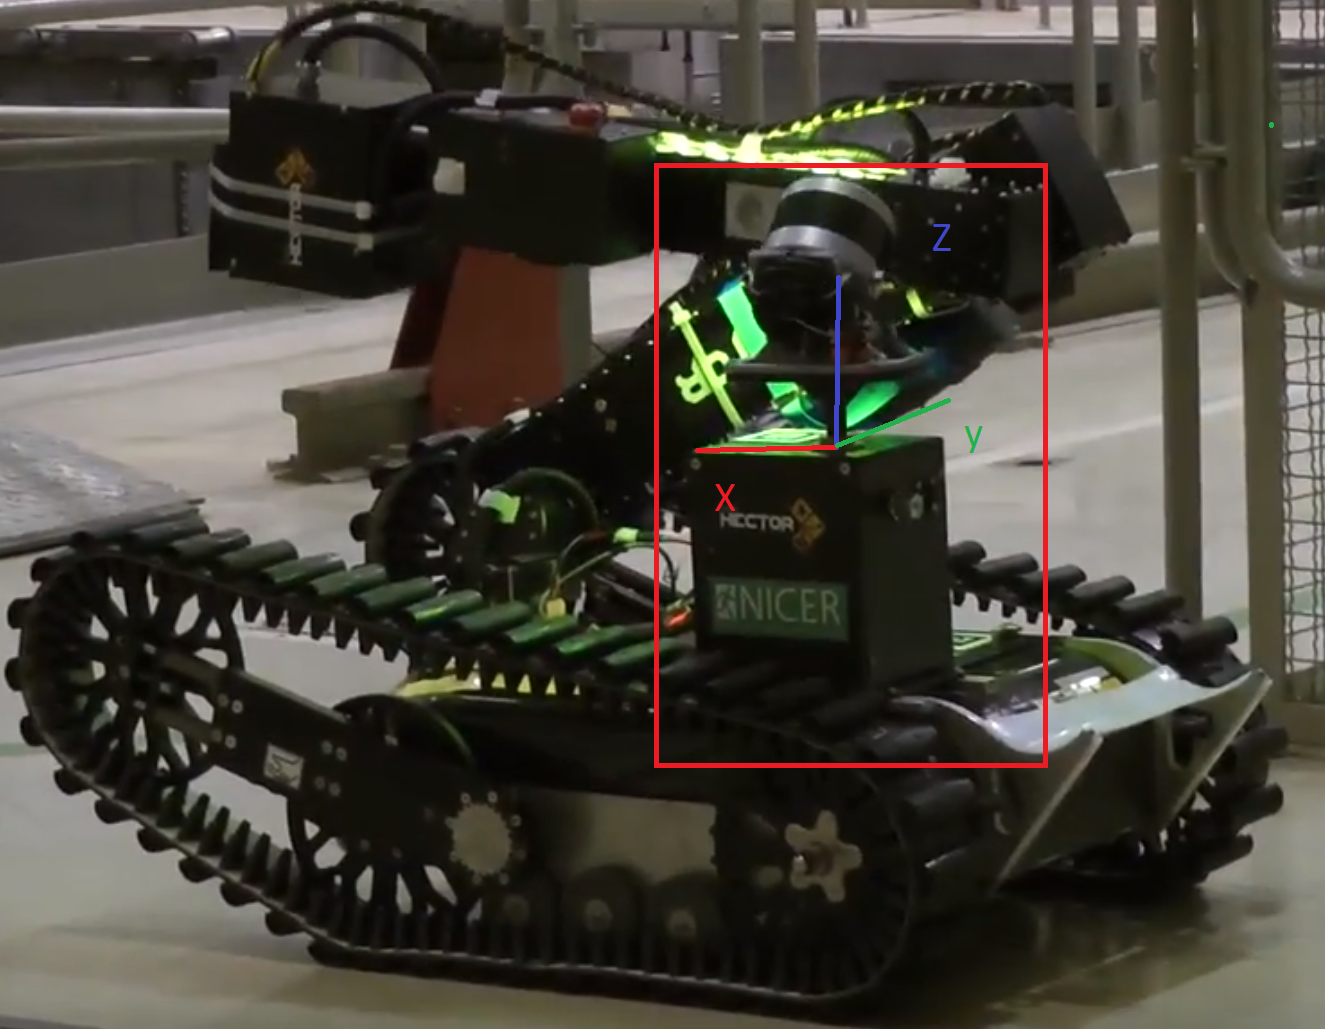
\includegraphics[width=0.7\textwidth]
	{resources/hector_cop.PNG}
	\caption[Roboter des Team Hector EnRicH]{Roboter des Team Hector an der EnRicH} \protect\cite{hector}
	\label{fig:hector}
\end{figure}

Im stationären Zustand kann durch diese Konfiguration keine Verbesserung der Auflösung erreicht werden. Die Auflösungen bleiben erhalten, sind jedoch nun entsprechend der Neigung um 45$^\circ$ verschoben. Durch die Neigung des Sensors wird der Raum nicht gleichmäßig vermessen. Die räumliche Vermessung wird auch hier erst mit der Rotation um die Z-Achse ermöglicht. Es kann während einer Umdrehung somit durch die Neigung von 45$^\circ$ und dem 30$^\circ$ Kegel des Sensors eine Abdeckung in der Vertikalen von 240$^\circ$ erreicht werden. Die horizontale Abdeckung bleibt hierbei weiterhin 360$^\circ$, da der Sensor die interne Rotation vollführt.

Gegenüber einer festen nicht drehenden Lösung besitzt diese Konfiguration somit den Vorteil, dass Messpunkte, welche sich zwischen den Laserstrahlen befinden, durch Drehen erreichen lassen. Dabei wird der 30$^\circ$ Messkegel durch die Rotation ständig im vertikalen Bereich hin- und hergeschoben.

Auch bei dieser Betrachtung  muss die Umdrehungsgeschwindigkeit der Konstruktion bedeutend langsamer als die interne Umdrehungsgeschwindigkeit des Sensor sein. Die Auflösung bei dieser Konstruktion ist direkt zur Umdrehungsgeschwindigkeit abhängig. 
Des Weiteren muss bei dieser Konfiguration die Translation, d.h. die Bewegung des Roboters, noch separat betrachtet werden.  

Im Vergleich zum Projekt der IMM entstehen bei dieser Konfiguration weniger Messpunkte in Richtung des Roboters und in in Richtung Z-Achse (himmelwärts). Dies ist für Raum interne Messungen unvorteilhaft. Für die Messung im freien Feld ist diese Konfiguration besser geignet, sofern sich keine  hohe Objekte nahe dem Sensor befinden.
 	
\subsection{Schlussfolgerung}
An der \ac{EnRicH} 2017 nutzen mehrere Teams den Velodyne VLP-16 mit unterschiedlichen Konfigurationen. Die zwei betrachteten Konfigurationen nutzen die Möglichkeit einer endlos drehenden mechanischen Konstruktion. Im Unterkapitel \ref{sec:Antriebsmoeglichkeiten} werden mögliche Antriebsmöglichkeiten für eine solche Konstruktion evaluiert. Eine endlos drehende Konstruktion benötigt eine spezielles Handling der Kabelführung, daher wird im Unterkapitel \ref{sec:Schleifring} die Möglichkeit eines Schleifrings beschrieben. Beide Konfiguration besitzen Vor- und Nachteile bei der Umgebungserkennung. Um eine möglichst detaillierte Umgebungswolke zu erstellen müssen vorwiegend Translation und Rotation um die Drehachse kompensiert werden.
  

\section{Software}
\label{sec:Software}
In diesem Kapitel wird die notwendige Software beschrieben. Es erläutert einerseits das \ac{ROS} und dessen Funktion im Projekt. Daneben werden kurz weitere Softwareapplikationen und -packages erwähnt, welche für die Aufgabenstellung nützlich sind.

\subsection{ROS Robot Operating System}
\label{subsec:ROS}
Die gesamte Kommunikation mit Sensoren und Aktoren findet auf dem Packbot mit \ac{ROS} statt. Da das 3D-Laser-Modul auf dem Packpot, wie auch selbstständig funktionieren soll, ist ROS nicht zwingend einsetzbar. Dennoch wurde für die Aufgabenstellung ROS gewählt. Im Zusammenhang mit Velodyne und 3D Mapping bietet ROS neben Visualisierungtools und  bereits bestehender Treiber-Packages auch die Integrationen der Point Cloud Library (PCL). Dies ist eine umfangreiche Library, welche viele Funktionen und Codebeispiele bereit stellt. 

Grundsätzlich wird \ac{ROS}, wegen seiner Nähe zu Linux Distributionen, auf einem Ubuntu Betriebssystem aufgesetzt und ist ein Software-Framework, dass die Programmiersprachen C++ und Python nutzt. Diese in 2007 entwickelte Open Source Software erhielt in den letzten Jahren ständig neue und überarbeitete Versionen. In der nachfolgenden Abbildung sind die aktuellen Distributionen ersichtlich.

\begin{figure}[H]
	\centering
	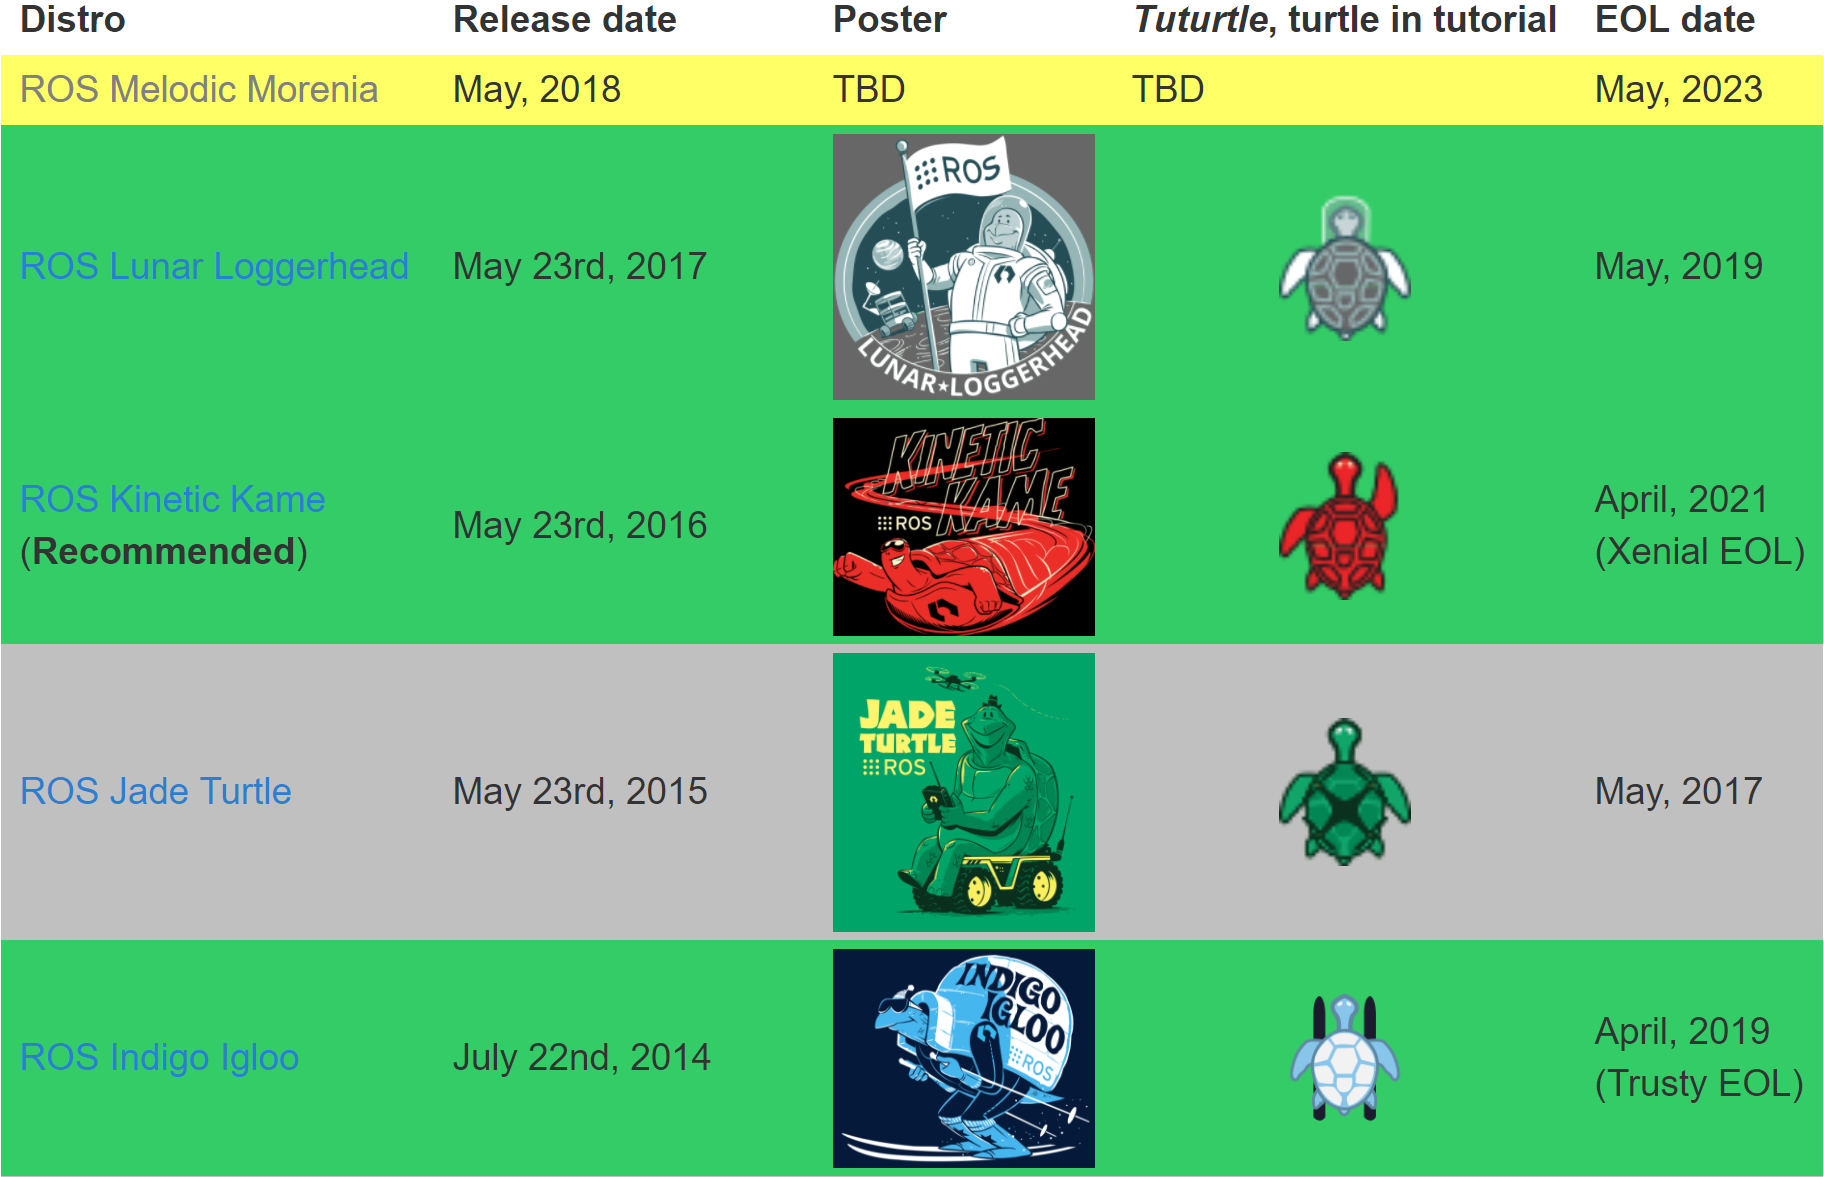
\includegraphics[width=0.4\textwidth]{resources/rosdistos.PNG}
	\caption[aktuelle Distributionen von ROS]{aktuelle Disttributionen von ROS {\cite{ROSprojects}}}
	\label{fig:rosdistros}
\end{figure} 

Die Empfehlung von ROS und diversen Literaturen liegt hierbei bei der neusten Distribution ROS "Kinetic Kame". \cite{ROSprojects} Es handelt sich hierbei um eine Langzeitversion von ROS, welche bis 2021 Unterstützung bietet. Im Zug der ersten Versuchen mit ROS wurde auf einem Laptop mit AMD64-Architektur gearbeitet. Auf diesem wurde ROS Kinetic Kame vollumfänglich ermöglicht. Für das 3D-Lasermodul wird jedoch ein einbaubaren Einplatinencomputer benötigt, welche im \ref{sec:Datenverarbeitung} genauer betrachtet werden. 

Während der Einarbeitung mit Kinetik Kame konnten einige Nachteile der Distribution festgestellt werden. Es wurde festgestellt, dass diverse Packages nur für AMD64-Architekturen zur Verfügung stehen und nicht für ARM-Architekturen. Dies ist ein wesentlicher Nachteil, da die meisten Einplatinencomputer mit ARM-Architekturen arbeiten.

\subsection{Velodyne Package}
Wie bereits im vorherigen Kapitel erwähnt besitzt ROS ein Treiber-Package für den Velodyne VLP-16. In der Abbildung \ref{fig:rosgraph} ist der Aufbau dieses Treibers mit dem ROS-Tool rqt-graph visualisiert.

\begin{figure}[H]
	\centering
	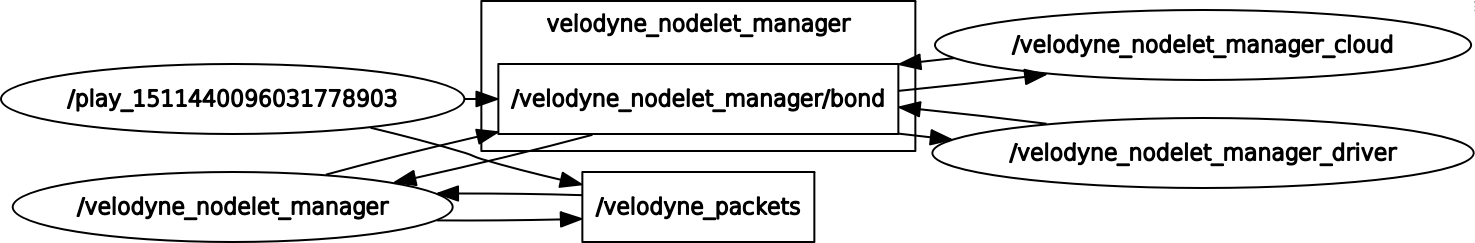
\includegraphics[width=1\textwidth]{resources/rosgraph.png}
	\caption[Velodyne Treiber aus rqt-graph ]{Velodyne Treiber aus rqt-graph }
	\label{fig:rosgraph}
\end{figure} 




\section{Datenverarbeitung}
\label{sec:Datenverarbeitung}
Um die Datenmenge zu verarbeiten und die Ansteuerung der Komponenten zu realisieren, eignen sich Einplatinencomputer. Einplatinencomputer besitzen den Vorteil, dass sie gegenüber üblichen Mikroprozessoren grössere Speichermöglichkeiten, höhere Prozessorleistung und bootbare Betriebssysteme ermöglichen. Gegenüber \ac{XPC} besitzen sie den Vorteil, dass sie Hardware näher sind, indem sie direkt ansteuerbare Pins besitzen (GPIO). Aus diesem Grund werden nachfolgend diverse Einplatinencomputer betrachtet. Kriterien bei der Auswahl eines geeigneten Boards sind Prozessorleistung, Preis, Ethernet-Schnittstelle, Speichermöglichkeit, GPIO Verfügbarkeit und die verbaubare Dimension. 

\subsection{Raspberry Pi 2 \& 3}
\label{subsec:Raspberry}
Das Raspberry Pi ist eines der bekanntesten Einplatinencomputer und bietet daher eine grosse Community. Da bereits ein Raspberry Pi 2 zur Verfügung gestanden ist, konnten die ersten Erfahrungen mit einem Raspberry Pi gemacht werden. Das Raspberry bietet zusammen mit ROS Kinetic Kame und Ubuntu Mate LTS 16.04 eine mögliche Lösung für die Datenverarbeitung. Das Raspberry Pi 2 bzw. 3 basiert auf einem Broadcom \ac{SOC} und ist mit einem ARM Cortex A7 bzw. A53 Prozessor mit vier Kernen ausgestattet. Die Taktfrequenz liegt bei diesen lediglich bei 1.2 GHz. Beide Modelle besitzen 1 GB RAM. Das Betriebssystem wir auf einer \ac{SD}-Card gebootet.

\subsection{Banana Pi M3}
\label{subsec:BananaPi}
Der Banana Pi M3 bietet zur Zeit (Stand Oktober 2017) die höchste Performance bei Einplatinencomputern mit ARM-Architektur durch den Allwinner A83T Achtkern-Prozessor, der mit 1.8 GHz taktet. Neben USB-Anschlüssen bietet es eine SATA-USB-Schnittstelle, die den internen 8 GB \ac{eMMC}-Speicher um bis zu 2 TB erweitern lässt. Es bietet auch direkt integrierte WLAN-Schnittstellen, sowie eine RJ45 Gigabit Netzwerkschnittstelle. Zum Betreiben des Banana PI M3 benötigen man ein 5V DC-Netzteil. Der Preis eines BananaPi M3 liegt momentan bei ca 90. Franken. Da im Zusammenhang mit Banana Pi M3 und Ubuntu mehrfach Komplikationen und Probleme veröffentlicht werden. \cite{banana}; 

 
\subsection{Odroid C2 \& XU4} 
\label{subsec:Odroid}
In diversen Literaturen (siehe \cite{ROSprojects} Kapitel 4) werden neben dem Raspberry Pi, Odroid Boards als empfohlene Einplatinencomputer aufgelistet. Dabei stehen die aktuelle Modelle Odroid-C2 oder Odroid-XU4 zur Verfügung. Sie bieten eine höhere Prozessorleistung, 1.5 GHz bzw. 2 GHz mit je 2 Gigabyte \ac{RAM}. Betribssysteme können via \ac{SD} oder \ac{eMMC} gebootet werden. Beide Boards sind jedoch noch nicht lange auf dem Markt und bieten in vielen Anwendungen nur Beta-Versionen. Vor allem die Unterstützung von Ubuntu LTS 16.04 ist nicht restlos geklärt. Der Preis dieser Boards ist um die 80 - 90 Franken.

\subsection{Up Board Squared} 
\label{subsec:Lattepanda}
Der Up Board Squared Einplatinencomputer unterscheidet sich wesentlich von den bisherig betrachteten Boards. Der Prozessor arbeitet nicht mit ARM-Architektur, sondern mit AMD64-Architektur. Somit können Ubuntu und ROS Distributionen vollumfänglich genutzt werden. Es besitzt mit Intel Pentium ein vier kerniger Prozessor und taktet mit 2.5 GHz. Zusätzlich bietet es einen separaten 500 MHz \ac{GPU} und bis zu 8 GB \ac{RAM}. Es bietet neben USB, eine zweifache RJ45-Schnittstelle und auch ein GPIO Pin Layout, welches dem Raspberry Pi entspricht. Der Preis eines Up Board Squared kostet je nach Ausführung zwischen 180-380 Fr.

\subsection{Schlussfolgerung}
\label{subsec:Schlussfolgerung}
Für die Aufgabenstellung eignet sich lediglich das Raspberry Pi 2 oder 3, um ROS mit Ubuntu LTS 16.04 zu betreiben. Das Banana Pi und die Odroid Boards sind im Kriterium Speichermöglichkeit und Prozessorleistung besser geeignet, können jedoch wegen fehlender Betriebsystem-Kompatibilität nicht genutzt werden. Einzig das Up Board Squared bieten in fast allen Kriterien eine denkbare Lösung. Aus Kostengründen wurde jedoch das Raspberry Pi als genügend bewertet.  

\section{Antriebsmöglichkeiten}
\label{sec:Antriebsmoeglichkeiten}
Um das Produkt um eine Achse drehen zu lassen, müssen Motoren eingesetzt werden. Nachfolgend sind zwei verschiedene Motorenarten geschildert, um die Einsatzmöglichkeit zu klären. Wichtige Kriterien für die Aufgabenstellung sind einerseits die Ansteuerung und die Dimension. Anderseits muss die Möglichkeit bestehen die Winkeländerung zu eruieren. 

\subsection{Schrittmotor}
\label{subsec:Schrittmotor}
Der Schrittmotor ist eine Antriebsmöglichkeit, welche für das Projekt in Frage kommt. Es gibt sehr kostengünstige und kompakt dimensionierte Motoren dieser Art. Ein interessanter Aspekt ist das gezielt Steuern des Motors. Durch einen Stromimpuls bewegt sich ein Schrittmotor nur einen festgelegten Winkelschritt weiter. Er kann bereits ohne zusätzliche Sensorik definierte Schritte anfahren, aus denen die Winkeländerung eruiert werden kann. Schrittmotoren besitzen die Eigenschaft, dass in der Ruhelage ein Haltemoment entsteht. Diese Eigenschaft wird jedoch für die Aufgabenstellung nicht zwingend benötigt. 

Nachteilig für die Aufgabenstellung am Schrittmotor ist der höhere Stromverbrauch, vor allem zum Aufbringen des Haltemoments. Da nur ein Schritt vollführt werden kann, wenn das entsprechende Drehmoment nicht überschritten wird, müsste dieses sorgfältig berechnet werden. Ein bedeutender Nachteil im Zusammenhang mit der Aufgabenstellung ist, dass durch Schrittverluste die Winkeländerung nicht mehr quantitativ ermittelt werden kann.
Ein weiterer Nachteil ist das verhältnismäßig hohe Gewicht. Dies ist kein Kriterium für die Aufgabenstellung, sollte jedoch bei der Realisierung beachtet werden.

Um mit einem Mikrocontroller einen Schrittmotor anzusteuern, empfiehlt sich ein Schrittmotorentreiber. Mit solchen Treibern lässt sich der Motor mittels 2 Steuerpins rotieren. Um die Drehgeschwindigkeit zu senken, bieten diese Treiber die Möglichkeit, die Schritte in 2, 4, 8 und 16 Teilschritte zu senken,um dadurch eine feinere Bewegung zu ermöglichen. 

\subsection{Gleichstrommotor}
Als Alternative zum Schrittmotor bietet sich ein üblicher Gleichstrommotor. Diese Motoren sind für viele Einsatzbereiche geeignet und es gibt sie in verschiedenen Grössen und Umdrehungszahlen. Im Gegensatz zu Schrittmotoren laufen Gleichstrommotoren kontinuierlich, aufgrund eines Stroms, der durch die Wicklungen fliesst. Nachteilig ist somit, dass weder die genaue Anzahl Umdrehungen noch die momentane Phasenlage bekannt ist. Es gibt jedoch eine Vielzahl an Möglichkeiten diese zu eruieren. Einerseits gibt es die Möglichkeit mittels Hall-Sensoren oder mittels Quadraturencodern, die aktuelle Drehrichtung und die Drehzahl zu ermitteln. Um dies zu ermöglichen, braucht es zusätzlich einen Vierquadrantensteller (H-Brücke), sowie eine Sensorlogik, damit der Sensor mittels \ac{PWM} angesteuert werden kann. Im Preissegment bis 40 Fr. gibt es leistungsfähige Gleichstrommotoren für den Anwendungsbereich.

\section{Absolute Positionsbestimmung}
\label{sec:position}
Damit beim 3D Mapping eine feste Koordinatenachse erstellt werden kann, benötigt eine drehende Konstruktion eine absolute Positionsbestimmung. Nachfolgend sind Varianten erläutert, welche sich dafür eignen.

\section{LED und Photodiode }
Eine simple Variante ist der Einsatz einer LED, welche im rotierenden Teil konstant leuchtet. Dabei wird die Photodiode an den stationären Teil angebracht und als Nullpunkt genutzt. Durch das Licht der LED wird ein Strom an der Photodiode übertragen und dies kann mit einer einfachen Beschaltung über einen GPIO gemessen werden. Nachteilig bei dieser Variante ist der Lichtkegel der LED. DIE LED müsste so verbaut werden, dass ein fokussierter Lichtstrahl auf die Photodiode fällt. Zudem ist diese Variante sehr stark abhängig von Umgebungslicht. Ansonsten kann der Nullpunkt stark abweichen. Diese Variante bedingt das mittels einer weiteren Komponente die Winkeländerung gemessen werden kann.

\section{Sensor QRE 1113}
Eine weiter ähnliche Variante ist der Einsatz eines QRE 1113 Sensor. Dieser Sensor baut auf dem Prinzip der Infrarotreflektion auf. Dabei werden dunkle Oberflächen schlechter reflektiert, als helle Oberflächen. Diese Eigenschaft wird genutzt, um den Nullpunkt zu detektieren. Auch diese Variante bedingt das mittels eines weiteren Komponente die Winkeländerung gemessen werden kann.
Eine weitere Überlegung ist die Aneinanderreihung von diesen Sensoren. Dies bietet die Möglichkeit einen Quadraturencoder Binär oder Gray-Code, wie in Abbildung \ref{fig:Encoder} zu realisieren.

\begin{figure}[H]
	\centering
	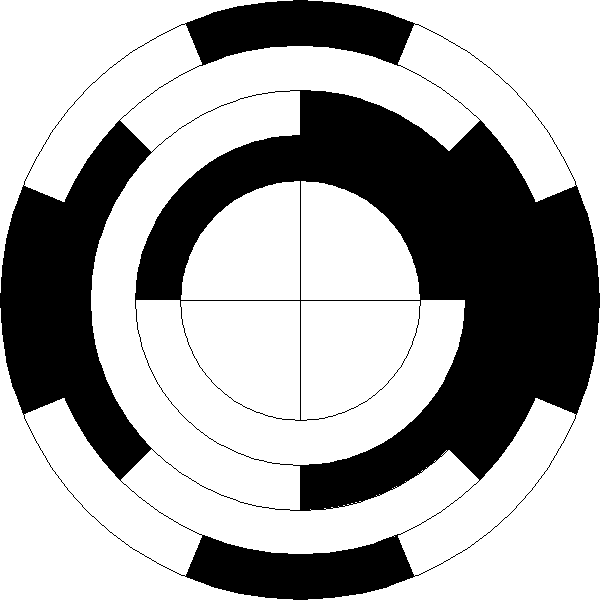
\includegraphics[width=0.4\textwidth]{resources/encoder.png}
	\caption[Quadraturencoder mit 4 Sensoren]{Quadraturencoder mit 4 Sensoren}
	\label{fig:Encoder}
\end{figure} 

 Es können mit N Sensoren 2$^N$ Zustände unterschieden werden. Aus der Auflösung kann der Winkel berechnet werden. Für diese Aufgabe werden jedoch auch N GPIOs benötigt. Auch diese Variante ist stark abhängig vom Umgebungslicht und zusätzlich können die einzelnen Sensoren einander durch Streuung beinflussen. Um dies zu minimieren sollte eine solche Variante mittels Gray-Code realisert werden, damit nur immer eine gleichzeitige Zustandsänderung stattfindet. Die Abtastung der Zustände müsste nach dem Nyquist-Shannon-Abtasttheorem mit mindestens doppelter Abtastfrequenz gemessen werden.  

\section{Speisung und Verkabelung}
\label{sec:Speisung und Verkabelung}

\subsection{Abwärtswandler}
\label{subsec:Abwaertswandler}
Der Abwärtswandler D24V50F5 von Pololu eignet sich sehr gut für die Stromversorgung von Einplatinencomputer. Er bietet eine stabile 5V-Ausgangsspannung bis zu einer ausgangsseitigen Belastung von 8 Ampere. Der Wirkungsgrad beläuft dabei auf über 90 Prozent bei einer eingesetzten Betriebsspannung von 12 Volt. Diese Angaben gehen aus Abbildung \ref{fig:D24V50F5} hervor, die aus dem Datenblatt des Abwärtswandler entstammen.

\begin{figure}[H]
	\centering
	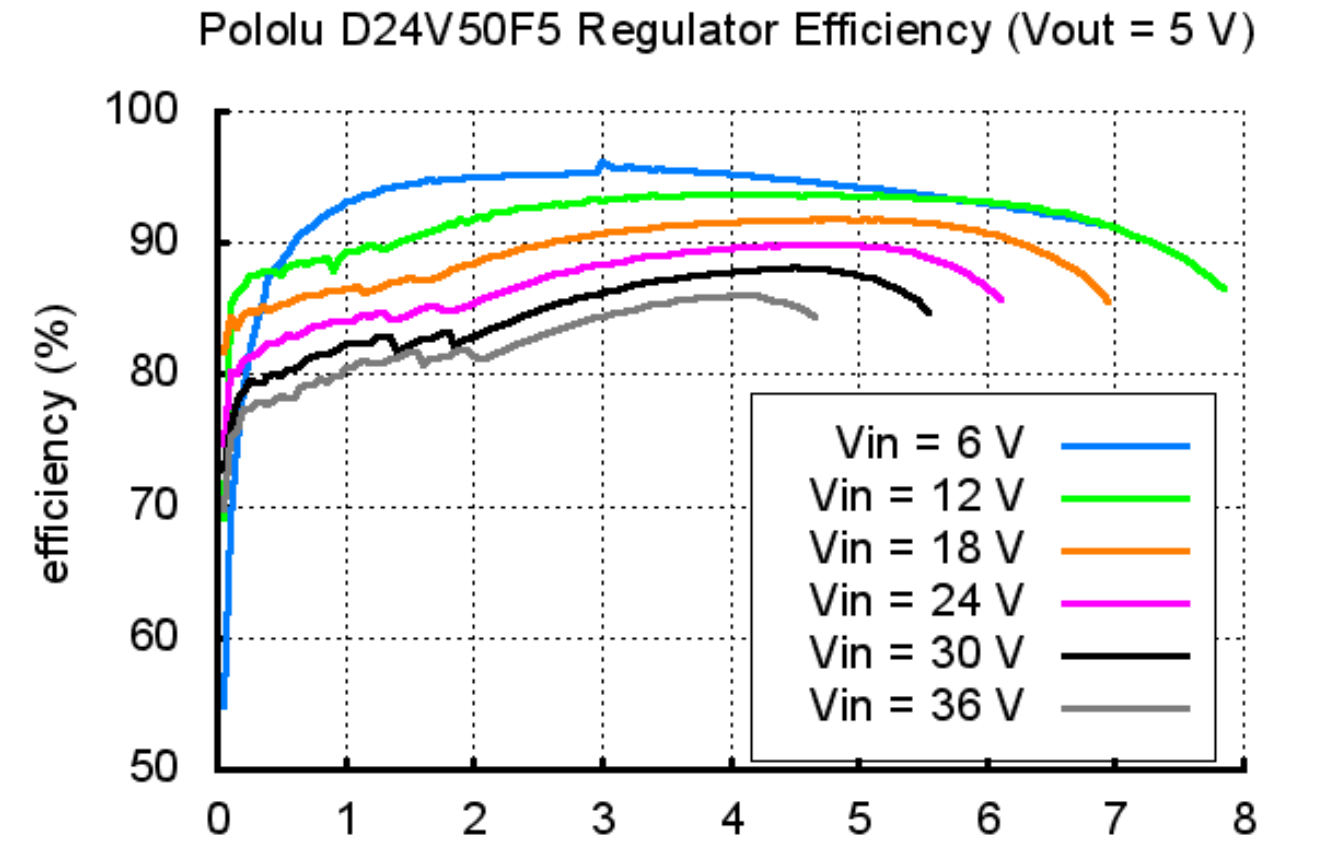
\includegraphics[width=0.5\textwidth]
	{resources/D24V50F5.PNG}
	\caption[Wirkungsgrad D24V50F5]{Wirkungsgrad D24V50F5 \protect\cite{D24V50F5}}
	\label{fig:D24V50F5}
\end{figure}

\subsection{Schleifring}
\label{subsec:Schleifring}
Da übliche Kabel nur für einige wenige Verdrehungen ausgelegt sind und so bei endlos drehenden Vorrichtungen kaputt gehen würden, werden Schleifring als Drehübertrager eingesetzt. Ein Schleifring überträgt das Eingangssignal über eine Bürste und bildet somit einen Gleitkontakt. Da vermehrt nicht nur Speisung, sondern auch Datenübertragung über Schleifringe geführt werden, wächst dieses Sortiment stetig. Es gibt bereits einige wenige Hersteller aus dem amerikanischen und asiatischen Markt, welche Ethernet-Übertagung für Schleifringe vertreiben. Ein Ethernet-Schleifring, der zusätzlich Leistungsübertragung bis 5A zulässt kostet nach Abklärungen bei diversen Herstellern zwischen 120 - 500 Fr.  


\section{Zwischenfazit}
\label{ZwischenfazitInfo}
Für die Einarbeitung in das Projekt ist die Informationsbeschaffung bzw. Recherche ein wesentlicher Bestandteil. Dabei werden wichtige Grundlagen für die Konzeption erstellt. Mittels Schrittmotoren oder Gleichstrommotoren kann der Velodyne gedreht werden. Für die Datenverarbeitung stehen mehrere Einplatinencomputer zur Verfügung, dabei muss jedoch die Integration in das System gewährleistet sein. Für endlos drehende Konfigurationen wird zusätzlich ein Schleifring benötigt, da ansonsten die Kabelführung nicht gewährleistet ist. 